\section{Related Work}
\label{sec:related}
\begin{figure}[t]
    \centering
    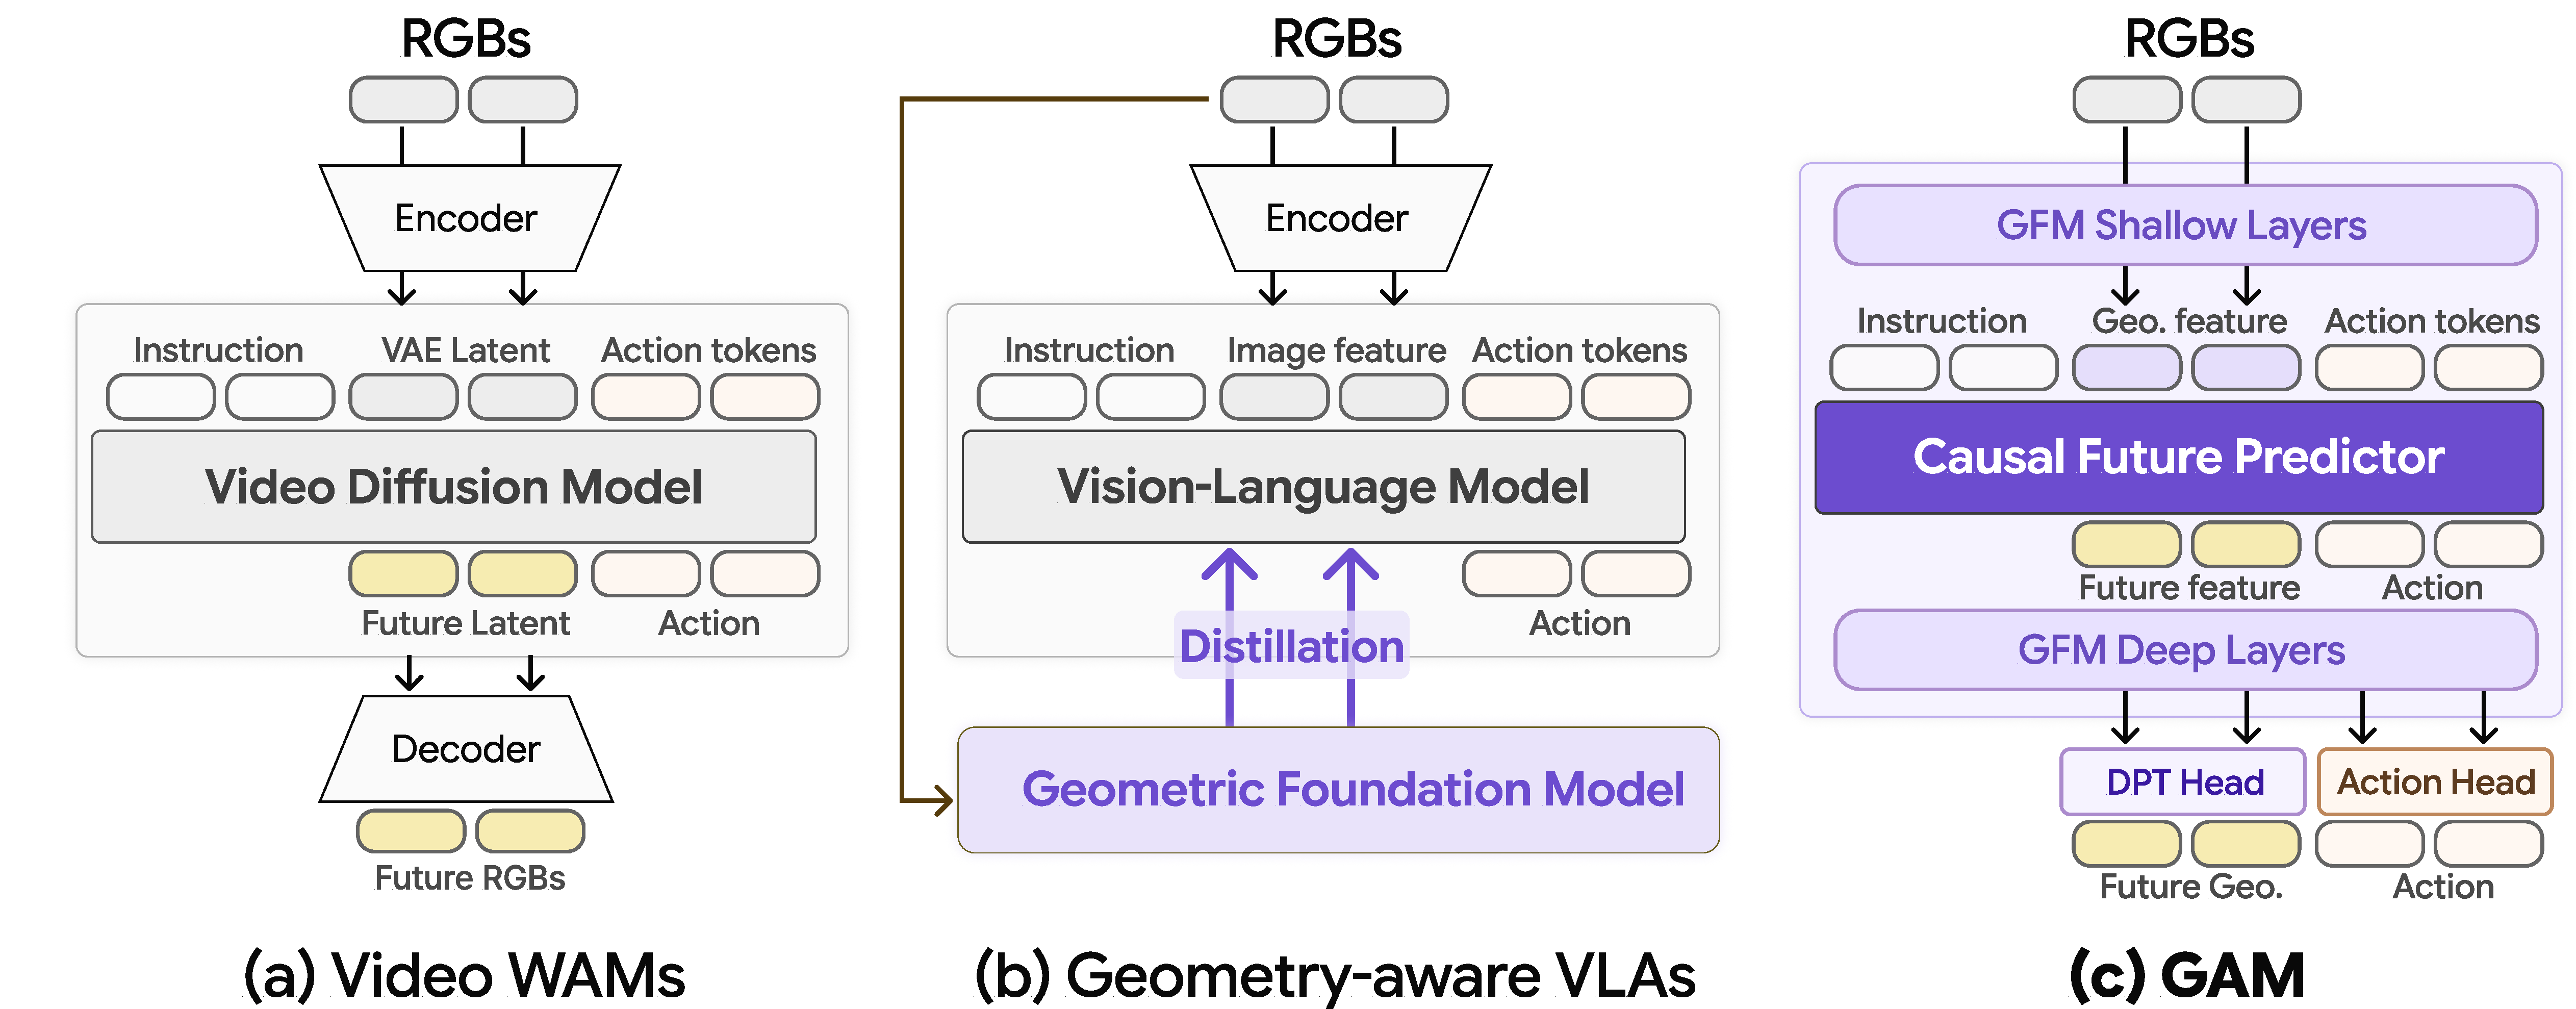
\includegraphics[width=1\linewidth]{figures/compare2.pdf}
    \caption{\textbf{(a) Video WAMs}~\citep{kim2026cosmos,pai2025mimic, ye2026world} operate in 2D pixel space, predicting future latents and actions via video diffusion. \textbf{(b) Geometry-aware VLAs}~\citep{li2025spatial, sun2026rocket} predict actions using a VLA with passive feature distillation from an external GFM. \textbf{(c) GAM (ours)} unifies perception, geometry prediction, and action decoding by inserting a geometric world model inside a single GFM.}

    \vspace{-10pt}
    \label{fig:intuition}
\end{figure}
\noindent\textbf{Vision-Language-Action Models.}  
Vision-language-action models (VLAs) adapt a pretrained vision-language model (VLM) into a robot policy. Early works~\citep{zitkovich2023rt, kim2024openvla} autoregressively decode discrete action tokens from a finetuned VLM. This paradigm is extended through parallel decoding~\citep{openvla_oft}, flow-matching action experts~\citep{black2024pi_0, pi05, shi2025hi}, diffusion-based action heads~\citep{liu2025rdt}, frequency-space action tokenizations~\citep{pi0_fast}, and compact open-source VLMs~\citep{nora,bai1others}.
This line of work extends large generalist foundation models for humanoid and embodied control~\citep{bjorck2025gr00t, team2025gemini, cheang2025gr, yang2025magma}, to spatial-representation variants~\citep{qu2025spatialvla}, and to refinements in training and post-training ~\citep{univla, riptvla, worldvla}.
While these VLAs leverage strong open-vocabulary recognition to produce policies, they rely solely on 2D image priors and therefore lack 3D understanding. To address this, recent works~\citep{li2025spatial, sun2026rocket, abouzeid2025geoaware} attempt to align intermediate VLA features with geometric foundation model. However, they do not fully exploit the geometric understanding of geometric foundation model backbone.
 
\noindent\textbf{World Action Models for Robot Manipulation.}
World action models are trained to predict future states in order to learn a policy. One branch builds on large pretrained video generation models~\citep{agarwal2025cosmos}, fine-tuning them to jointly predict future frames and actions~\citep{kim2026cosmos, pai2025mimic, ye2026world}, arguing that the benefit of such co-training stems primarily from training-time supervision rather than test-time future imagination~\citep{ye2026world, pi0_fast}. A second branch keeps the visual backbone frozen and trains a separate temporal predictor in its feature space for planning via model-predictive control~\citep{zhou2024dino, assran2025v}, with related work using implicit future-latent alignment as an auxiliary training signal~\citep{zheng2025flare}. However, these video backbones encode only 2D image-space priors, which do not explicitly resolve depth, scale, or occlusion. GAM instead predicts in the latent space of a geometric foundation model that encodes rich 3D priors, while inheriting from both branches the paradigm of using future prediction as a training signal.


\noindent\textbf{Geometric Foundation Models for Manipulation.} Geometric foundation models (GFMs)~\cite{wang2025vggt, lin2025depth, wang2025pi, keetha2025mapanything} infer dense 3D structures from multi-view images and have recently served as perceptual substrates for robot policies. Early approaches integrate GFMs with VLAs as frozen feature extractors via representation alignment~\citep{li2025spatial, sun2026rocket}, direct encoder replacement~\citep{abouzeid2025geoaware, qian2025gp3}, or point-cloud fusion~\citep{sun2025geovla}. Moving beyond static extraction, recent concurrent works adopt GFMs for predictive control: \citet{song2026robotic} utilizes the GFM to jointly predict actions and \emph{current}-frame 3D properties, while \citet{xu2026action} employs the GFM with a diffusion policy to co-denoise future action chunks and 3D latents. GAM departs from these paradigms in two ways: (1) action and future-scene predictions are jointly modeled within a single autoregressive token sequence rather than separated heads or diffusion processes, and (2) the GFM's deep blocks are explicitly repurposed to decode predicted \emph{future} tokens rather than merely processing observed ones.
